\documentclass[14pt,twocolumn,letterpaper]{extarticle}


\setlength{\textheight}{9.075in}
\setlength{\textwidth}{6.875in}
\setlength{\columnsep}{0.3125in}
\setlength{\topmargin}{-0.3in}
\setlength{\headheight}{0in}
\setlength{\headsep}{0in}
\setlength{\parindent}{1pc}
\setlength{\oddsidemargin}{-.304in}
\setlength{\evensidemargin}{-.304in}

\usepackage{times}
\usepackage{epsfig}
\usepackage{graphicx}
\usepackage{amsmath}
\usepackage{amssymb}
\usepackage{courier}
\usepackage{tabularx}
\usepackage{makecell}
\usepackage{booktabs}

\usepackage{indentfirst}
\setlength{\parindent}{1em}

\usepackage[breaklinks=true,bookmarks=false]{hyperref}
\setcounter{page}{1}
\begin{document}

\title{A Study On Adam And AdamW}
\author{D11949006 Wei-Lun Chen \\ R11921118 Yong-Tai Qiu}
\date{}
\maketitle

\section{Introduction}
The field of machine learning has witnessed the advent of numerous optimization algorithms, among which the Adam and AdamW optimizers stand out due to their unique characteristics and widespread use. Despite their extensive application, certain features within these optimizers still call for comprehensive exploration and validation. Therefore, this research sets out to achieve three primary objectives centered around these optimizers.\par
Firstly,we strive to gain a comprehensive understanding of the Adam and AdamW optimizers. We seek to delve into their operational principles, understand the theoretical underpinnings that govern their functioning, and explore their common usage in machine learning tasks. This foundational understanding will set the stage for subsequent investigations and pave the way for our next objectives.\par
Our second goal is to evaluate the significance of the bias correction feature intrinsic to the Adam optimizer. This bias correction, integral to Adam's functionality, is designed to offset any underestimation of the gradient moments during the initial stages of training. However, the practical implications of this feature on model performance are not fully understood. We propose to probe into the role of bias correction through extensive experimentation and detailed analysis. Our study design includes varying learning rates and beta values while observing the impacts with and without bias correction.\par
Finally, our third aim is to draw comparisons between L2 regularization in Adam and weight decay in AdamW. AdamW was conceived as a solution to the issues found with weight decay in Adam, yet the distinction between the two and their consequent impact on model performance remain somewhat hazy. Our research intends to illuminate these subtle differences, offering strong empirical evidence to validate the distinction. This objective includes experiments with varying lambda values to understand the effects on L2 regularization and AdamW.\par
Through this study, we aspire to enrich our understanding of these optimizers and offer significant insights that may inform optimization decisions in machine learning projects. Our experimental outcomes, documented through loss and accuracy measures, will provide robust evidence to support our conclusions.

\section{Methods}
In our research, we conducted a comparative evaluation using a Convolutional Neural Network (CNN) model performing classification tasks on the MNIST dataset. To maintain a balanced comparison, we kept consistent the model architecture, initial weight settings, training epochs, batch size, and the loss function across all experimental setups. We scrutinized four unique settings of the optimizer: the conventional Adam optimizer, a modified Adam version without bias correction, Adam incorporating L2 regularization, and AdamW. These configurations were meticulously chosen to explore the impacts of bias correction and different weight decay methods on the performance of the model.\par
For every optimizer setup, we trained our CNN model across 100 epochs with a batch size of 64. To ensure consistency in the starting point, we initiated the model with identical random seeds across all conditions, guaranteeing uniform initial weights. The loss function employed was Cross Entropy Loss.\par
We undertook the training with three distinct learning rates $\left(\gamma\right)$ – 1e-3, 1e-4, and 1e-5 – applied to each of the four optimizers. This procedure enabled us to study the variation in the model's performance under different learning rates spanning the optimizers. In all scenarios, the beta parameters $\left(\beta_{1}\ \text{and}\ \beta_{2}\right)$ were set at 0.9 and 0.999, respectively, while the epsilon $\left(\epsilon\right)$ was established at 1e-8. These configurations were selected to be in sync with commonly used values in existing literature.\par
Finally, we integrated weight decay in the Adam with L2 regularization and the AdamW optimizers, standardizing the decay factor $\left(\lambda\right)$ to 0.01 in both instances. This facilitated us to draw direct comparisons between the effects of L2 regularization and weight decay decoupling on the model's performance.\par
Through this experimental design, we were able to systematically investigate the comparative impacts of bias correction and different weight decay methods on the performance of a CNN model in image classification tasks.



\section{Results}
Table 1 shows our experimental settings. In Experiment 1-1 and Experiment 1-2, we want to know whether or not bias correction will affect the accuracy under different learning rates and different betas? \par In Experiment 2, I want to know whether it will affect the accuracy of Adam and AdamW under different lambda (weight decay)?

\begin{table*}[ht!]
\centering
\caption{Experimental Settings}
\newcolumntype{Y}{>{\centering\arraybackslash}X}
\newcolumntype{Z}{>{\centering\arraybackslash}p{.35\textwidth}}
\begin{tabularx}{\textwidth}{|Y|Z|Z|}
\hline
\textbf{Hyperparameter} & \textbf{Exp1} & \textbf{Exp2} \\
\hline
Optimizer & \makecell{Adam \\ Adam w/o Bias Correction} & \makecell{Adam (L2) \\ AdamW} \\
\hline
Learning Rate ($\gamma$) & 1e-3, 1e-4, 1e-5 & 1e-4 \\
\hline
\makecell{Beta Parameters \\ ($\beta_1$, $\beta_2$)} & (0.9, 0.999), (0.99, 0.999) & (0.9, 0.999) \\
\hline
Epsilon ($\epsilon$) & 1e-8 & 1e-8 \\
\hline
Decay Factor ($\lambda$) & - & 1e-2, 1e-3, 1e-4 \\
\hline
\end{tabularx}
\label{tab:exp_settings}
\end{table*}

Figure 1 shows the results of Experiment 1-1, represents the verification accuracy of Adam with or without bias correction under the same learning rate and different betas. \par

It can be found that under same learning rate, different betas, the with or without of bias correction has little effect on the accuracy rate.\par

\begin{figure}[ht!]
\centering
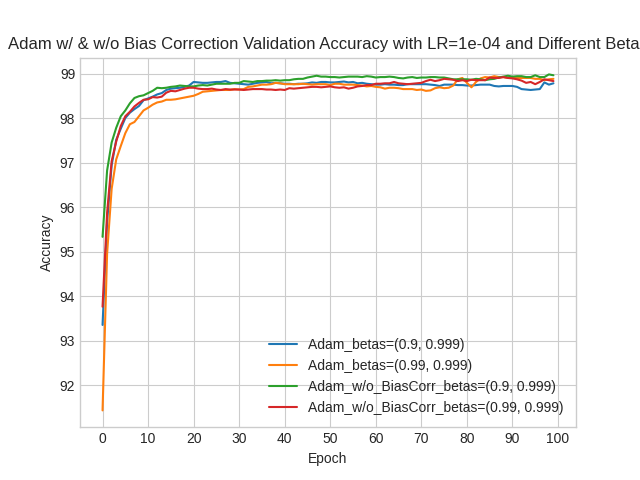
\includegraphics[width=\linewidth] {adam_with_and_without_bias_correction-1e-04-validation_accuracy.pdf}
\caption{Adam with and without bias correction with learning rate 1e-04 and different betas validation accuracy}
\label{adam_with_and_without_bias_correction-1e-04-validation_accuracy}
\end{figure}

We only show results for learning rate 1e-4 here, but in fact learning rates 1e-3, 1e-5 have similar results.\par

Figure 2 shows the results of Experiment 1-2, represents the verification accuracy of Adam with or without bias correction under the same betas and different learning rate. \par 
It can be found that under same betas, different learning rate, the with or without of bias correction has little effect on the accuracy rate.

\begin{figure}[ht!]
\centering
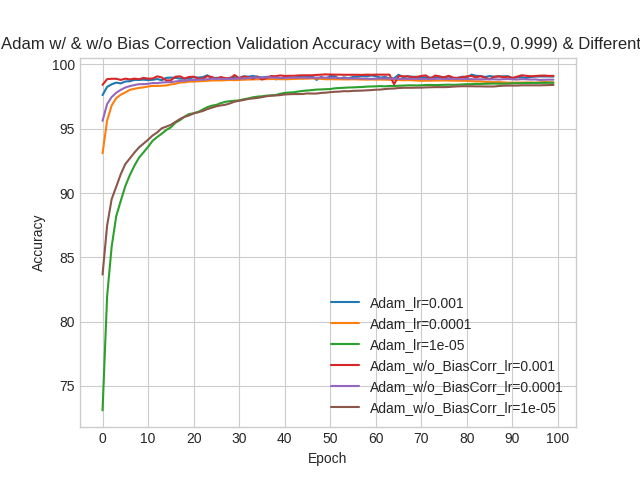
\includegraphics[width=\linewidth] {adam_with_and_without_bias_correction-(0.9, 0.999)-validation_accuracy.pdf}
\caption{Adam with and without bias correction with betas (0.9, 0.999) and different learning rate validation accuracy}
\label{adam_with_and_without_bias_correction-(0.9, 0.999)-validation_accuracy}
\end{figure}

We only show results for betas (0.9, 0.999) here, but in fact betas (0.99, 0.999) have similar results.\par


Figure 3 shows the results of Experiment 2, represents the verification accuracy of Adam with L2 and adamW under different lambdas(weight decay).\par

We can found in Experiment 2 that if Adam's L2 is larger, the accuracy rate will be smaller. In addition, the Adam+L2 scheme will lead to Suboptimal optimization process, and the L2 size of AdamW seems to have little effect on the accuracy.

\begin{figure}[ht!]
\centering
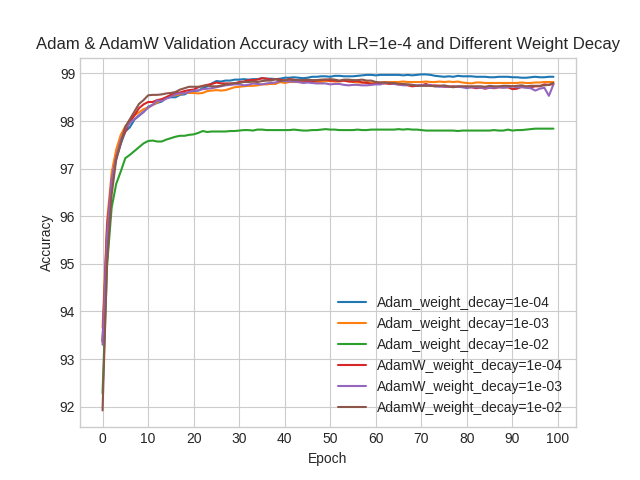
\includegraphics[width=\linewidth] {adam_and_adamw_diff_weight_decay-validation_accuracy.pdf}
\caption{Adam and AdamW with different weight decay validation accuracy}
\label{adam_and_adamw_diff_weight_decay-validation_accuracy}
\end{figure}



\section{Discussion and Conclusions}

Let's break down and discuss each experiment individually: \par

\textbf{Experiment 1-1 and Experiment 1-2:}
The results indicate that the presence or absence of bias correction does not significantly impact the accuracy rate, regardless of the learning rate and betas used. This suggests that, in these experiments, bias correction does not play a crucial role in improving the model's accuracy. It could imply that bias correction may not be essential in certain contexts or that other factors overshadow its influence on model performance. Further research is necessary to explore the underlying reasons for this observation. \par

\textbf{Experiment 2:}
The findings from Experiment 2 reveal that higher L2 regularization parameter in Adam leads to lower accuracy rates. This could be attributed to the stronger constraint imposed on the model's weights by larger L2 regularization, limiting the model's expressive power and consequently affecting its performance.  The weight decay and L2 regularization may reach equivalence under some conditions still are slightly different concepts and should be treated differently otherwise can lead to unexplained performance degradation or other practical problems.

However, the optimal value of the regularization parameter depends on the specific dataset and problem at hand. Therefore, in practical applications, fine-tuning the regularization parameter may be necessary to achieve optimal performance.

In summary, these conclusions highlight the effects of bias correction and L2 regularization in different scenarios. Further investigation is needed to gain a deeper understanding of these observations and to determine the generalizability of the findings across various datasets and models.

\bibliographystyle{ieee}
% \bibliography{egbib}

\end{document}
%%% Local Variables:
%%% mode: latex
%%% TeX-master: t
%%% End:
